\documentclass[../AdvancementSummary.tex]{subfiles}

\begin{document}



%%%%%%%%%%%%%%%%%%%%%%%%%%%%%%%%%%%%%%%%%%%%%%%%%%%
\section{Model Development}
%%%%%%%%%%%%%%%%%%%%%%%%%%%%%%%%%%%%%%%%%%%%%%%%%%%
\label{sec:ModelDev}

We create a generic model of a disordered protein using a simplified $\theta$-solvent freely-jointed chain (FJC) from polymer physics. This model requires only specifying a number of rods (N) and a length per rod (Kuhn length, $\delta$). The FJC consists of N rigid rods of length $\delta$ which are allowed to perform a random walk where the only constraints are the chain length and connections. In our simulation, the FJC is allowed to explore its configuration space through randomized movements. The FJC model tracks where each joint is located, making steric interactions with the ligand easy to simulate compared to using the continuous WLC model. The ligand is simulated as an idealized sphere which may interact with the FJC. We compute quasi-equilibrium statistics of the chain and its bound or unbound ligands using a Monte Carlo (Metropolis) Algorithm. 

We model the polymer in the canonical ensemble, i.e. equilibrium. Steric occlusion of binding sites by the rest of the chain therefore gives rise to a change in $K_D$. We can compute the difference in $K_D$ between two states, e.g. fully phosphorylated compared to unphosphorylated. From detailed balance, we have $K_D \equiv \koff/\kon$, which allows us to compute the change in $K_D$ as follows: 

\begin{align} 
\frac{k_{on}}{k_{off}} &= \mbox{exp} \left( \frac{-\Delta G}{k_B T}\right) \\
\frac{K_{D_1}}{K_{D_2}} &= \frac{\frac{1}{\mbox{exp} \left( \frac{-\Delta G_1}{k_B T}\right) }}{\frac{1}{\mbox{exp} \left( \frac{-\Delta G_2}{k_B T}\right)}} \\ 
&= \frac{\mbox{exp} \left( \frac{-\Delta G_2}{k_B T} \right)}{\mbox{exp} \left( \frac{-\Delta G_1}{k_B T} \right)} \\
&= \mbox{exp} \left(\frac{\Delta G_1-\Delta G_2}{k_B T}\right) \\. 
&= \mbox{exp} \left( \frac{(E_1-T S_1)-(E_2-T S_2)}{k_B T} \right) \\
&= \mbox{exp} \left(\frac{S_2-S_1}{k_B}\right) \\
&=\mbox{exp}\left(\frac{(S^2_{on}-S^2_{off}) - (S^1_{on}-S^1_{off})}{k_B} \right) \\
&= \mbox{exp} \left( \frac{(k_B \mbox{ln} (\frac{\Omega_2 P_2}{\Omega_2}))-(k_B \mbox{ln}(\frac{\Omega_1 P_1}{\Omega_1})}{k_B} \right) \\
\frac{K_{D_1}}{K_{D_2}} &= \frac{P_2}{P_1}\\
\end{align}  

where $G_j=E_j-TS_j$ is the free energy of binding in the free or rigid state, $S_j = k_B \mbox{ln} W$ is the entropy of binding, where W is the number of microstates and $P_j$ is the probability in the canonical ensemble that the configuration allows for binding. We let $\Omega$ be the total number of microstates, with $\Omega_1 P_1$ being the microstates available when the ligand is bound and $\Omega_2 P_2$ is the number of microstates available when the polymer is rigid. We also note $E_2 = E_1$ since we are working at equilibrium. 

For example, we can consider the change in $K_D$ between a fully rigid polymer, where all binding sites are available and $K_D = K_{D_R}$, compared to a floppy, unstructured polymer, where binding site availability depends on the conformation of the polymer and $K_D = K_{D_F}$. Then we calculate the change in $K_D$ as above, but since the rigid state always allows binding, we may write $P_R =1$. 

\begin{align} 
\frac{K_{D_F}}{K_{D_R}}  &= \frac{\frac{1}{\mbox{exp} \left( \frac{-\Delta G_F}{k_B T}\right) }}{\frac{1}{\mbox{exp} \left( \frac{-\Delta G_R}{k_B T}\right)}} \\ 
&= \frac{P_R}{P_F}\\
\frac{K_{D_F}}{K_{D_R}} &=\frac{1}{P_F} \hspace{2cm} \text{assuming $P_R$ = 1} \\
\end{align}  

We define $P_{occ}$ as the probability that the region of space needed by the kinase domain is occupied by some of the polymer. Thus, $P_{occ}=1-P_F$. Our problem of interest is now reduced to computing the occlusion probability. 

\begin{equation}
\frac{K_{D_F}}{K_{D_R}} = \frac{1}{(1-P_{occ})}. \\
\end{equation}

We have already used this comparison as a possibility to account for the change in phosphorylation rates of the TCR $\zeta$ chain \cite{Mukhopadhyay2016}. We consider the generalized version for the rest of our work. 

Steric occlusion by the polymer will impact the ability of a ligand to localize to the binding site. Although entropic forces could also impact unbinding of the polymer, we assume this influence to be negligible compared to the change in $k_{on}$. Therefore, for the body of this work, we assume that the change in $K_D$ stems from a change in $k_{on}$.

We calculate the occlusion probability by computing how often a ligand is able to bind to an oriented sphere tangentially attached to the polymer. We define `able to bind' as when the specified sphere is empty of both other polymer segments and any surface constraints. To determine if a site is occluded in a given conformation, we check if any of the segment end points are located within the sphere of interest. If a surface is present, we also check if the ligand sphere crosses below the half-space surface designated at $z=0$. Given that the binding sphere is large compared to the Kuhn length, we assume the probability of tangential occlusion (where a segment has end points outside the sphere but part of the segment lies within) is negligible compared to end point occlusion. 


%%%%%%%%%%%%%%%%%%%%%%%%%%%%%%%%%%%%%%%%%%%%%%%%%%%
\subsection{Code Validation}
%%%%%%%%%%%%%%%%%%%%%%%%%%%%%%%%%%%%%%%%%%%%%%%%%%%
There are theoretical solutions for many aspects of the freely-jointed chain. This provides a basis with which to verify our code. 

\subsubsection{Root-mean-square end-to-end distance}
First, we look at the average end-to-end distance of the polymer (RMS). In our simulations, we normalize by the Kuhn length, so all simulations assume $\delta = 1$ and record all other parameters in units of Kuhn lengths. We know from polymer physics that the RMS should increase as $\delta \sqrt{N}$, which given $\delta = 1$, is just $\sqrt{N}$.

Average end-to-end distance (Root-mean-square end-to-end distance) \cite{Reeves2011}:
\begin{equation*}
\sqrt{\langle r_{ee}^2 \rangle} = \sqrt{N\delta^2} = \delta \sqrt{N}
\end{equation*}

\begin{figure}[H]
\begin{center}
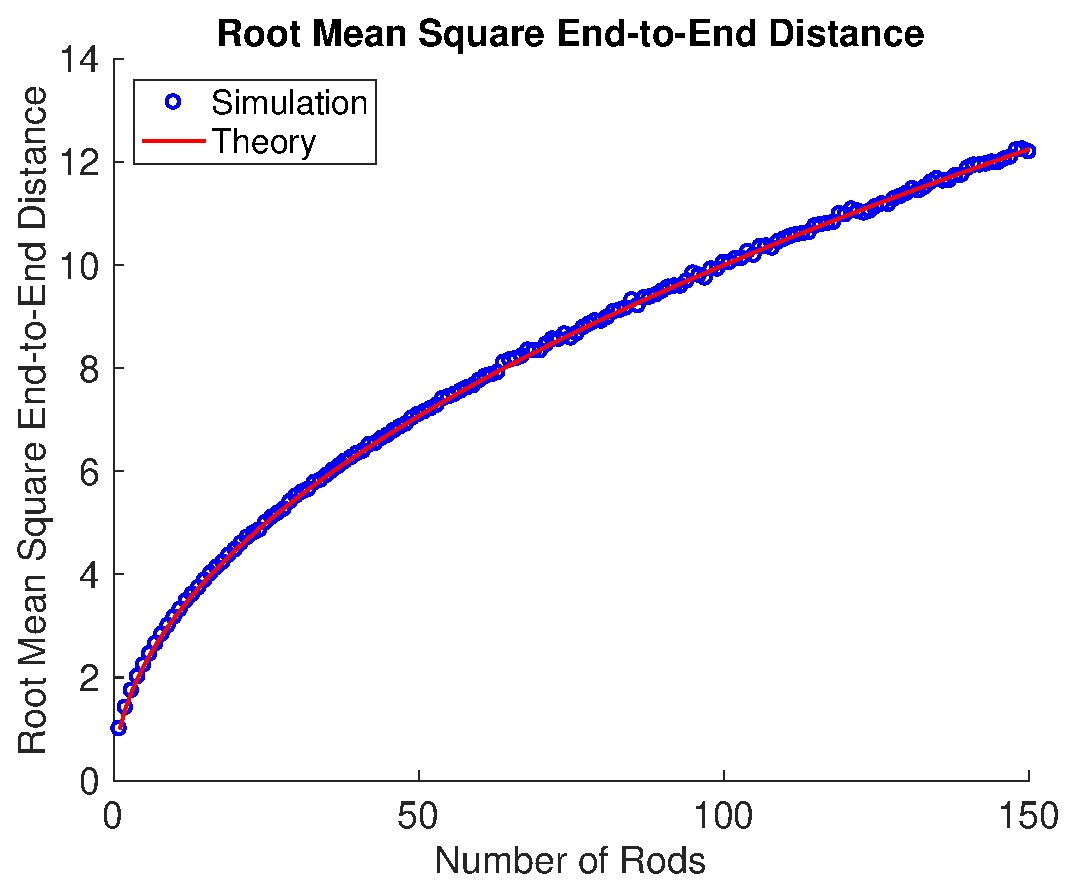
\includegraphics[width=0.5\linewidth]{ModelConfirmationFigures/RMSEndtoEnd.eps}
\caption{Theoretical root mean square end-to-end distance (red line) against simulated values (blue circles). \label{fig: RMS}}
\end{center}
\end{figure}

End-to-end distribution \cite{VanValen2009, Reeves2011}:
\begin{equation*}
P(r_{ee}) = 4\pi r^2 \left( \frac{3}{2\pi N \delta^2}\right)^{\frac{3}{2}}\text{exp}\left(\frac{-3r^2}{2N \delta^2}\right)
\end{equation*}


\begin{figure}[H]
\begin{center}
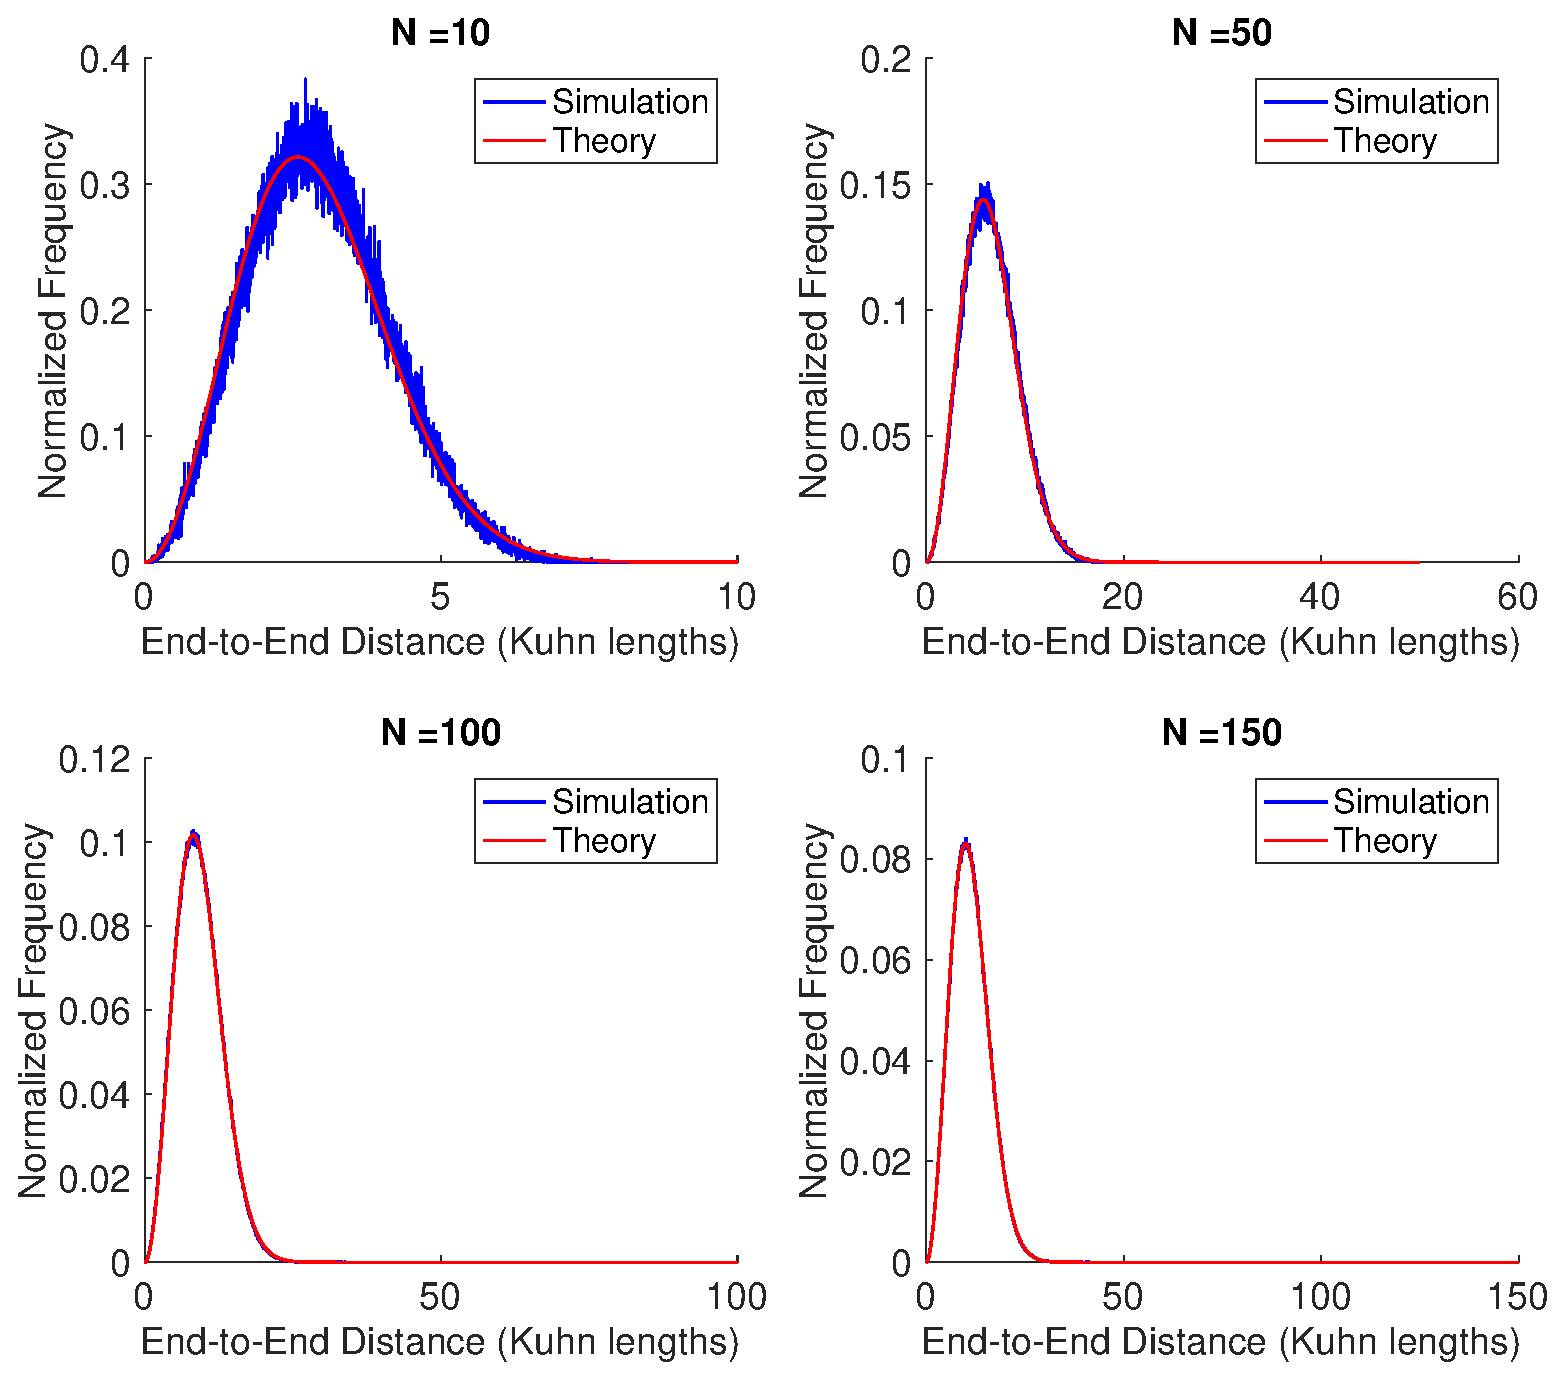
\includegraphics[width=0.8\linewidth]{ModelConfirmationFigures/ReeDistribution.eps}
\caption{Simulated end-to-end distance distribution (blue) against theoretical distribution (red) for multiple polymer lengths (N). \label{fig: ReeDist}}
\end{center}
\end{figure}

\subsubsection{Occlusion Probability of End Site VS Analytical Result}

We consider analytical solutions to the simplest case, where the ligand is attempting to bind at the end of the freely-jointed chain in free-space. The probability that a random walk over time 0 to $\delta N$, beginning at the edge of a sphere of radius, $R$, will cross into the sphere at any time is analogous to the probability the ligand is occluded by the freely jointed chain with $N$ segments and Kuhn length $\delta$. In order to solve this analytically, we must assume the random walk begins $\epsilon$ away from the sphere or it will always count as occluded. Then we may formulate as follows for the probability of survival, $p(\vec{x},t)$ when the random walk begins at a starting point, $r=R+\epsilon$:

\begin{equation}\label{eq: diffusion}
	\begin{cases}
		\frac{\partial p}{\partial t} = D \nabla^2 p, \hspace{2cm} p=0 \hspace{3mm}\text{at}\hspace{3mm} r=R\\
		p(\vec{x},0) = \delta(\vec{x}-(R+\epsilon))\\
	\end{cases}
\end{equation}

In order to get a finite estimate to compare, we consider the solution when $N\rightarrow \infty$.

 \begin{equation}\label{eq: analytic}
  	\begin{cases}
 	q(r)=\mathds{P}(\text{not hit sphere}|x(0)=r) \\
 	0=\frac{2}{r}q'(r)+q''(r) \\
 	q(R) = 0 \\
 	q(r) \rightarrow 1 \hspace{3mm}\text{as}\hspace{3mm} r \rightarrow \infty \\
 	\end{cases}
 \end{equation}

 We assume $\epsilon = 1$ Kuhn length and R measured in Kuhn lengths:

 \begin{equation}\label{eq: analyticSolution}
q(r) = 1-\frac{R}{r}\\
q(r) = 1-\frac{R}{R+1} \\
 \end{equation}
 
 We see that when we compare our simulated binding probability to the analytic solution, we get good agreement. This tells us both our code is working as desired and that N=100 is approximately $N \rightarrow \infty$.

 \begin{figure}[H]
 \begin{center}
 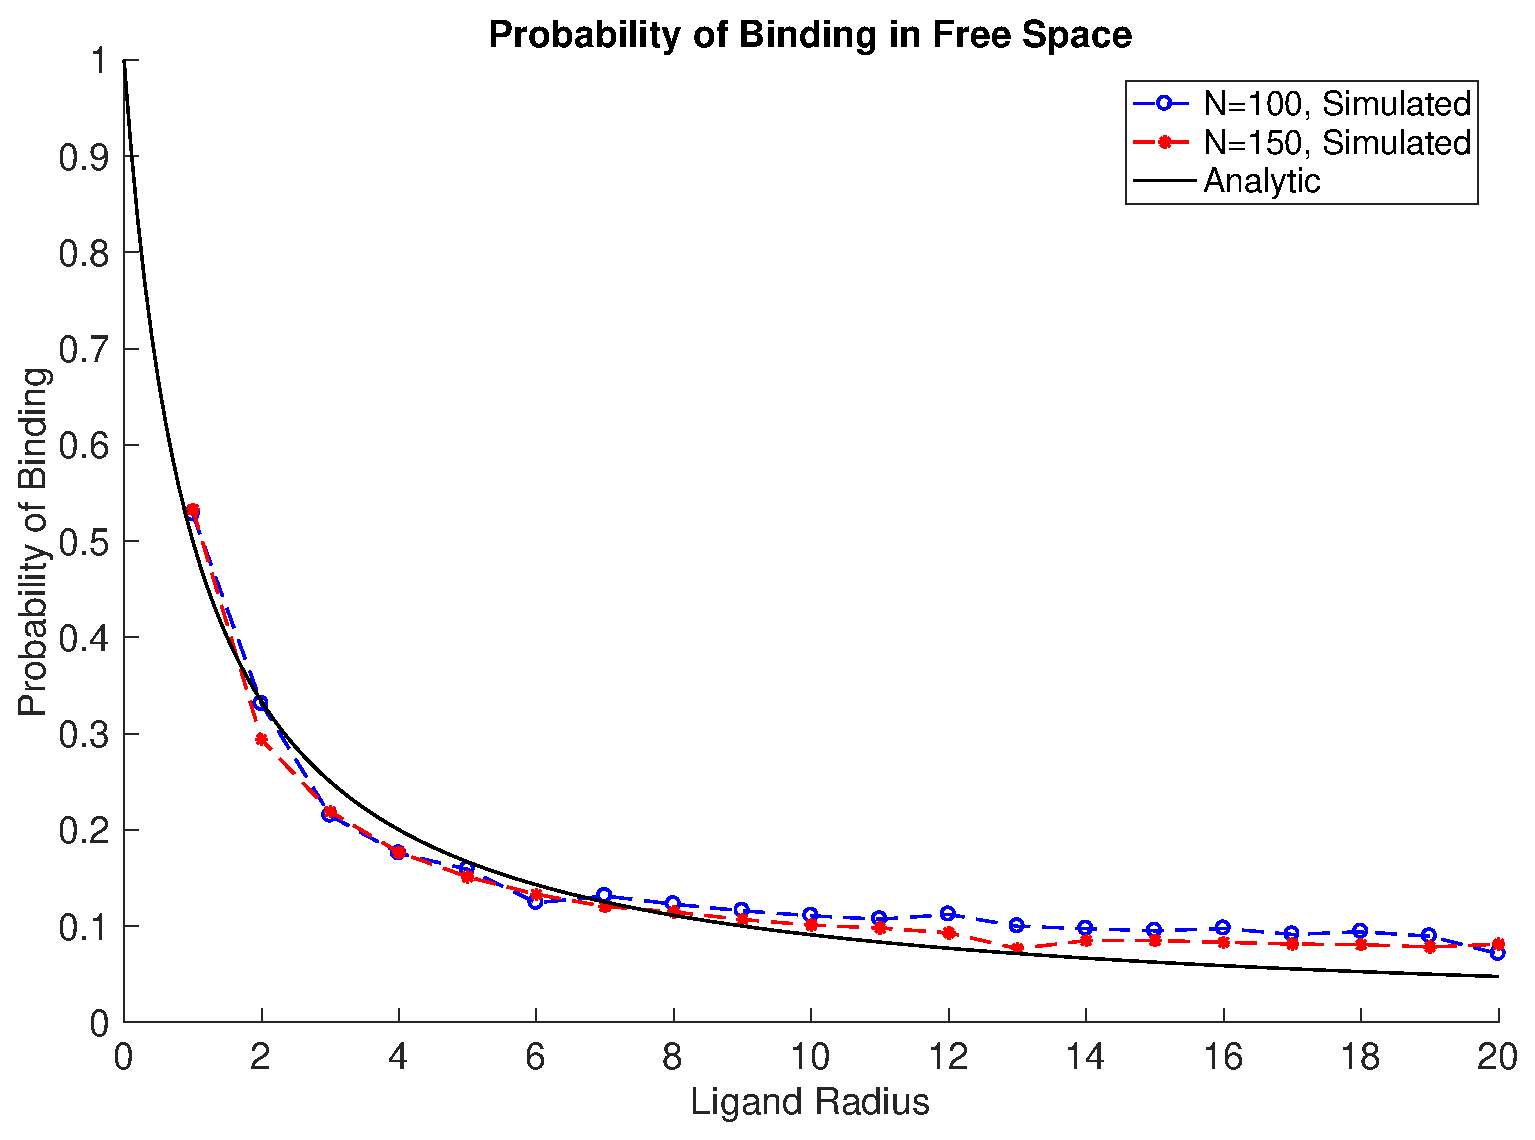
\includegraphics[width=0.7\linewidth]{ModelConfirmationFigures/BindingVSAnalyticN100N150.eps}
 \end{center}
  \caption{Analytic Solution \label{fig: AnalyticBinding}}
 \end{figure}





%%%%%%%%%%%%%%%%%%%%%%%%%%%%%%%%%%%%%%%%%%%%%%%%%%%
\subsection{Case Study: T Cell Receptor Zeta Chain}
%%%%%%%%%%%%%%%%%%%%%%%%%%%%%%%%%%%%%%%%%%%%%%%%%%%
\label{sec:ModelDevsubsec:TCR}
For the following study, we will focus on the mouse TCR CD3 $\zeta$ chain. The TCR CD3 $\zeta$ chain is a subunit of CD3 consisting of 164 amino acids. Of these, 21 are included in the signal peptide region of the protein. The remaining 143 amino acids make up the extracellular, transmembrane and cytoplasmic regions of the CD3 $\zeta$ chain. The cytoplasmic tail is an intrinsically disordered chain of 113 amino acids containing multiple phosphorylation sites, called ITAMs (immunoreceptor tyrosine-based activation motif). There are three ITAMs on the $\zeta$ chain, each containing two tyrosines. The tyrosine kinase Lck phosphorylates each tyrosine in the $\zeta$ chain. 

In mouse CD3 $\zeta$, the cytoplasmic tail spans residues 52-164 and the tyrosines are located at residues 72, 83, 111, 123, 142, 153. Therefore, if we were to renumber to begin at the beginning of the cytoplasmic tail, the region would be $N=113$ amino acids long, with tyrosines located at $i= 21, 32, 60, 72, 91, 102$ (UniProt, entry P24161). Given an assumption of 0.3\nm per Kuhn length (i.e. one Kuhn length is equivalent to one amino acid), then the tyrosines are similarly located along the 113 segments of the FJC.

Mouse Lck is composed of an SH3, SH2 and protein kinase domain connected by small loops. The domains are 61, 98, and 254 amino acids respectively (UniProt entry P06240). Using a protein molecular mass calculator, %(http://www.bioinformatics.org/sms/prot\_mw.html)
we calculate that the kinase domain is 29.08 kDa. If we assume a protein density of 1.41 $\mbox{g / cm}^3$ then we can estimate the volume of the kinase domain \cite{Fischer2004}:

\begin{equation*}
(29 \times 1000 \mbox{Da}) * (1.66\times10^{-27} \mbox{kg / Da}) * (1000 \mbox{g / kg}) / (1.41 \mbox{g / cm}^3) = 34 \nm^3.
\end{equation*}

If we then approximate the kinase domain as a sphere, then we can estimate a radius: 

\begin{align*}
V &= \frac{4}{3}\pi r^3 \\
34 \nm^3 &= \frac{4}{3} \pi r^3 \\
r &\approx 2 \nm \\
\end{align*}
%
%Measurements from the crystal structure of Lck suggest a volume of 45 $\nm^3$ for the kinase domain.\hl{Where did this come from?}This estimate is on the same order of magnitude as our previous estimate. Note also, if we recalculate the kinase radius using a volume of $45 \nm^3$, we estimate a radius of 2.2 \nm. 

We measure the maximal length of the kinase domain in PyMol from PDB 3LCK. Rounding up for error, we have a maximal distance of 58\AA. This gives a maximal spherical estimate with a radius of 2.9\nm, or about ten Kuhn lengths (Fig. \ref{fig: LckPyMol}a). If we instead measure rough length, width, and height for the kinase domain, we have measurements of 36.6\AA, 29.4\AA, and 45.1\AA respectively (Fig. \ref{fig: LckPyMol}b). From these we can estimate a sphere with volume corresponding to the volume of the rectangular prism with those dimensions. This estimates a sphere with radius 2.3\nm, or about eight Kuhn lengths. Based on all of these estimates, we choose to represent Lck with a radius of seven Kuhn lengths.


\begin{figure}[H]
\begin{center}
\begin{subfigure}{0.4\linewidth}
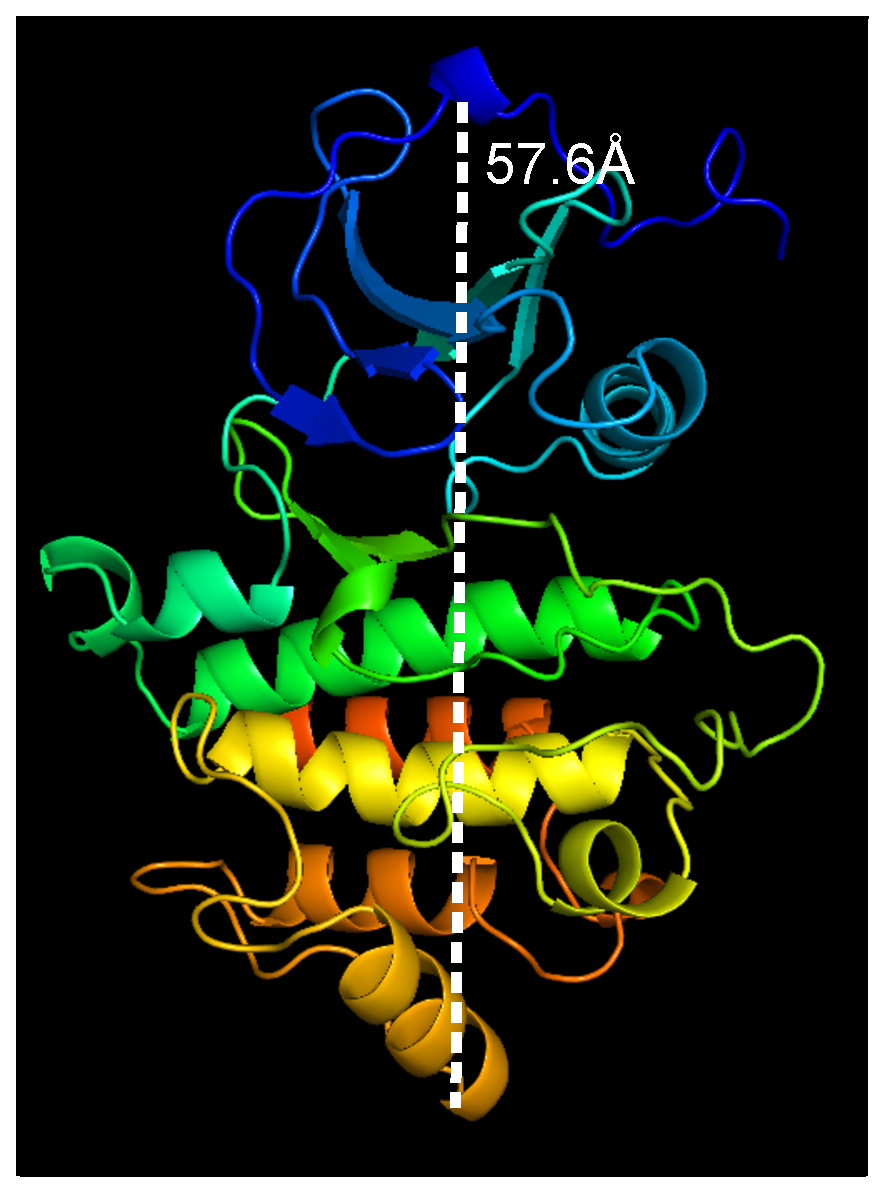
\includegraphics[width=\linewidth]{LckPyMol/Diagonal.eps}
\caption{}
\end{subfigure}
\begin{subfigure}{0.4\linewidth}
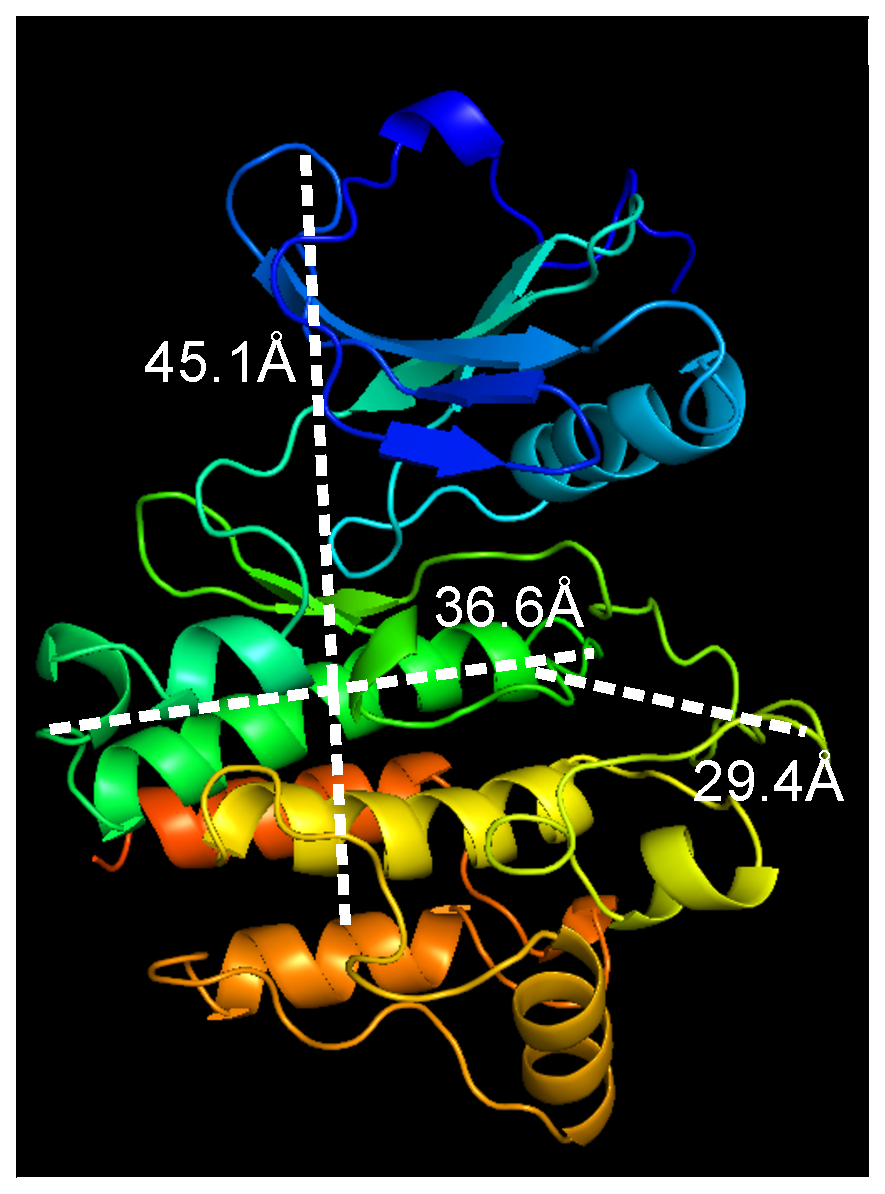
\includegraphics[width=\linewidth]{LckPyMol/LWD.eps}
\caption{}
\end{subfigure}
\end{center}
\caption{PDB 3LCK - kinase domain of Lck \label{fig: LckPyMol}}
\end{figure}



%\subsection{Possibly unnecessary stuff}
%
%\hl{where does this stuff go?}
%
%In this model, the FJC is allowed to pass through itself. However, this turns out to be unimportant. Although the disordered protein would have a nonzero bond width, this size would be small in comparison to the kinase volume and volume of exploration space. \hl{If you consider two thin strings in 3-dimensional space, they will almost never intersect.}  Therefore, we model our polymer with infinitely thin width. Since it is infinitely thin, the time when it would take on a conformation where it overlaps itself is negligible compared to the number of legal conformations it assumes.
%
%Additionally, we are only interested in the ensemble of configurations, not the dynamics. Therefore, the way the polymer achieves its conformations is unimportant to the results and any instances of self-intersection are negligible compared to the larger ensemble. Allowing the FJC to pass through itself, while unphysical, does not change the validity of our simulation.


%
%\subsection*{T Cell Receptor CD3 Zeta Chain Parameters}
%
%Our simulations currently assume all parameters are normalized by the Kuhn length. Therefore, to establish a Kuhn length of 0.3 $\nm$ to represent the CD3$\zeta$ chain, we set $N=113$. Now since our simulation measures ligand size in terms of Kuhn lengths, we estimate the ratio of the kinase radius to the Kuhn length size. Since we have an estimate of 2-2.2 $\nm$ radius, we use a radius of 7 Kuhn lengths for our simulations. Note also, that in the code, polymer joint numbering goes from 0 to N-1, so we input the tyrosines as $i=20,31,59,71,90,101$.

%Tyrosine kinases such as Lck bind to tyrosines on unstructured protein such as the ITAM domain on the T cell receptor zeta chain. There are multiple tyrosines on the zeta chain and it has been proposed that phosphorylation of one site influences the binding rate of kinase to other sites. 
%
%We assume that the unstructured domain transitions from a purely entropic freely jointed chain with Kuhn length $\delta = 0.3\nm$ and $N$ amino acids in total length, an approximation demonstrated to be valid for several unstructured domains \cite{Kutys:2010bk}, to a rigid rod. The kinase domain is assumed to be an impenetrable sphere of radius $r_{K}$. The kinase domain can only attach to the tyrosine, at site $i$, in one orientation relative to the tyrosine. (Rotational freedom of the kinase domain is irrelevant since it is unchanged between two ITAM states.)
%


%%%%%%%%%%%%%%%%%%%%%%%%%%%%%%%%%%%%%%%%%%%%%%%%%%%
\end{document}
%%%%%%%%%%%%%%%%%%%%%%%%%%%%%%%%%%%%%%%%%%%%%%%%%%%





